% Options for packages loaded elsewhere
\PassOptionsToPackage{unicode}{hyperref}
\PassOptionsToPackage{hyphens}{url}
%
\documentclass[
]{article}
\usepackage{amsmath,amssymb}
\usepackage{lmodern}
\usepackage{iftex}
\ifPDFTeX
  \usepackage[T1]{fontenc}
  \usepackage[utf8]{inputenc}
  \usepackage{textcomp} % provide euro and other symbols
\else % if luatex or xetex
  \usepackage{unicode-math}
  \defaultfontfeatures{Scale=MatchLowercase}
  \defaultfontfeatures[\rmfamily]{Ligatures=TeX,Scale=1}
\fi
% Use upquote if available, for straight quotes in verbatim environments
\IfFileExists{upquote.sty}{\usepackage{upquote}}{}
\IfFileExists{microtype.sty}{% use microtype if available
  \usepackage[]{microtype}
  \UseMicrotypeSet[protrusion]{basicmath} % disable protrusion for tt fonts
}{}
\makeatletter
\@ifundefined{KOMAClassName}{% if non-KOMA class
  \IfFileExists{parskip.sty}{%
    \usepackage{parskip}
  }{% else
    \setlength{\parindent}{0pt}
    \setlength{\parskip}{6pt plus 2pt minus 1pt}}
}{% if KOMA class
  \KOMAoptions{parskip=half}}
\makeatother
\usepackage{xcolor}
\usepackage[margin=1in]{geometry}
\usepackage{color}
\usepackage{fancyvrb}
\newcommand{\VerbBar}{|}
\newcommand{\VERB}{\Verb[commandchars=\\\{\}]}
\DefineVerbatimEnvironment{Highlighting}{Verbatim}{commandchars=\\\{\}}
% Add ',fontsize=\small' for more characters per line
\usepackage{framed}
\definecolor{shadecolor}{RGB}{248,248,248}
\newenvironment{Shaded}{\begin{snugshade}}{\end{snugshade}}
\newcommand{\AlertTok}[1]{\textcolor[rgb]{0.94,0.16,0.16}{#1}}
\newcommand{\AnnotationTok}[1]{\textcolor[rgb]{0.56,0.35,0.01}{\textbf{\textit{#1}}}}
\newcommand{\AttributeTok}[1]{\textcolor[rgb]{0.77,0.63,0.00}{#1}}
\newcommand{\BaseNTok}[1]{\textcolor[rgb]{0.00,0.00,0.81}{#1}}
\newcommand{\BuiltInTok}[1]{#1}
\newcommand{\CharTok}[1]{\textcolor[rgb]{0.31,0.60,0.02}{#1}}
\newcommand{\CommentTok}[1]{\textcolor[rgb]{0.56,0.35,0.01}{\textit{#1}}}
\newcommand{\CommentVarTok}[1]{\textcolor[rgb]{0.56,0.35,0.01}{\textbf{\textit{#1}}}}
\newcommand{\ConstantTok}[1]{\textcolor[rgb]{0.00,0.00,0.00}{#1}}
\newcommand{\ControlFlowTok}[1]{\textcolor[rgb]{0.13,0.29,0.53}{\textbf{#1}}}
\newcommand{\DataTypeTok}[1]{\textcolor[rgb]{0.13,0.29,0.53}{#1}}
\newcommand{\DecValTok}[1]{\textcolor[rgb]{0.00,0.00,0.81}{#1}}
\newcommand{\DocumentationTok}[1]{\textcolor[rgb]{0.56,0.35,0.01}{\textbf{\textit{#1}}}}
\newcommand{\ErrorTok}[1]{\textcolor[rgb]{0.64,0.00,0.00}{\textbf{#1}}}
\newcommand{\ExtensionTok}[1]{#1}
\newcommand{\FloatTok}[1]{\textcolor[rgb]{0.00,0.00,0.81}{#1}}
\newcommand{\FunctionTok}[1]{\textcolor[rgb]{0.00,0.00,0.00}{#1}}
\newcommand{\ImportTok}[1]{#1}
\newcommand{\InformationTok}[1]{\textcolor[rgb]{0.56,0.35,0.01}{\textbf{\textit{#1}}}}
\newcommand{\KeywordTok}[1]{\textcolor[rgb]{0.13,0.29,0.53}{\textbf{#1}}}
\newcommand{\NormalTok}[1]{#1}
\newcommand{\OperatorTok}[1]{\textcolor[rgb]{0.81,0.36,0.00}{\textbf{#1}}}
\newcommand{\OtherTok}[1]{\textcolor[rgb]{0.56,0.35,0.01}{#1}}
\newcommand{\PreprocessorTok}[1]{\textcolor[rgb]{0.56,0.35,0.01}{\textit{#1}}}
\newcommand{\RegionMarkerTok}[1]{#1}
\newcommand{\SpecialCharTok}[1]{\textcolor[rgb]{0.00,0.00,0.00}{#1}}
\newcommand{\SpecialStringTok}[1]{\textcolor[rgb]{0.31,0.60,0.02}{#1}}
\newcommand{\StringTok}[1]{\textcolor[rgb]{0.31,0.60,0.02}{#1}}
\newcommand{\VariableTok}[1]{\textcolor[rgb]{0.00,0.00,0.00}{#1}}
\newcommand{\VerbatimStringTok}[1]{\textcolor[rgb]{0.31,0.60,0.02}{#1}}
\newcommand{\WarningTok}[1]{\textcolor[rgb]{0.56,0.35,0.01}{\textbf{\textit{#1}}}}
\usepackage{graphicx}
\makeatletter
\def\maxwidth{\ifdim\Gin@nat@width>\linewidth\linewidth\else\Gin@nat@width\fi}
\def\maxheight{\ifdim\Gin@nat@height>\textheight\textheight\else\Gin@nat@height\fi}
\makeatother
% Scale images if necessary, so that they will not overflow the page
% margins by default, and it is still possible to overwrite the defaults
% using explicit options in \includegraphics[width, height, ...]{}
\setkeys{Gin}{width=\maxwidth,height=\maxheight,keepaspectratio}
% Set default figure placement to htbp
\makeatletter
\def\fps@figure{htbp}
\makeatother
\setlength{\emergencystretch}{3em} % prevent overfull lines
\providecommand{\tightlist}{%
  \setlength{\itemsep}{0pt}\setlength{\parskip}{0pt}}
\setcounter{secnumdepth}{-\maxdimen} % remove section numbering
\ifLuaTeX
  \usepackage{selnolig}  % disable illegal ligatures
\fi
\IfFileExists{bookmark.sty}{\usepackage{bookmark}}{\usepackage{hyperref}}
\IfFileExists{xurl.sty}{\usepackage{xurl}}{} % add URL line breaks if available
\urlstyle{same} % disable monospaced font for URLs
\hypersetup{
  pdftitle={Seccion 5.3 Transformaciones Para Linealizar Modelos},
  pdfauthor={Daniel Martinez},
  hidelinks,
  pdfcreator={LaTeX via pandoc}}

\title{Seccion 5.3 Transformaciones Para Linealizar Modelos}
\author{Daniel Martinez}
\date{}

\begin{document}
\maketitle

\begin{Shaded}
\begin{Highlighting}[]
\FunctionTok{library}\NormalTok{(MASS)}
\FunctionTok{library}\NormalTok{(latex2exp)}
\FunctionTok{library}\NormalTok{(ggplot2)}
\FunctionTok{library}\NormalTok{(tibble)}
\FunctionTok{library}\NormalTok{(dplyr)}
\end{Highlighting}
\end{Shaded}

\begin{verbatim}
## 
## Attaching package: 'dplyr'
\end{verbatim}

\begin{verbatim}
## The following object is masked from 'package:MASS':
## 
##     select
\end{verbatim}

\begin{verbatim}
## The following objects are masked from 'package:stats':
## 
##     filter, lag
\end{verbatim}

\begin{verbatim}
## The following objects are masked from 'package:base':
## 
##     intersect, setdiff, setequal, union
\end{verbatim}

\begin{Shaded}
\begin{Highlighting}[]
\FunctionTok{library}\NormalTok{(ggpubr)}
\FunctionTok{library}\NormalTok{(QuantPsyc)}
\end{Highlighting}
\end{Shaded}

\begin{verbatim}
## Loading required package: boot
\end{verbatim}

\begin{verbatim}
## Loading required package: purrr
\end{verbatim}

\begin{verbatim}
## 
## Attaching package: 'QuantPsyc'
\end{verbatim}

\begin{verbatim}
## The following object is masked from 'package:base':
## 
##     norm
\end{verbatim}

En el modelo habitual de regresión partimos del supuesto que hay una
relación lineal entre la variable \(y\) y los regresores. Sin embargo en
algunos casos esta suposición es inadecuada, puesto que por ejemplo si
observamos los gráficos de dispersión esta suposición puede no estarse
cumpliendo de manera evidente. Para poder solucionar este problema de no
linealidad, en algunos casos a estos modelos podemos hacerlos lineales,
usando una transformación adecuada.

Quizás nos preguntemos que comportamiento deberíamos observar para poder
encontrar una transformación que pueda linealizar el modelo. Antes de
mostrar algunos casos comunes en los que podemos transformar, veamos un
ejemplo de que va transformar un modelo que a primera vista no es
lineal, pero si podemos hacerlo lineal.

Consideremos la función \[y=\beta_0 e^{\beta_1 x}\varepsilon\] Esta
función como podemos ver no es linear, pero la podemos transformar en
una lineal si aplicamos un logaritmo, con lo que obtenemos
\[\ln{y}=\ln{\beta_0 e^{\beta_1 x}\varepsilon}=\ln{\beta_0}+\beta_1 x+\ln{\varepsilon}\]
Haciendo \(y'=\ln{y}\), \(\ln{\beta_0}=\beta_0'\),
\(\ln{\beta_1}=\beta_1'\) y \(\ln{\varepsilon}=\varepsilon'\), tenemos
el modelo \[y'=\beta_0'+\beta_1' x+\varepsilon'.\] Como podemos observar
en esta transformación estamos tomando el logaritmo del error, de modo
que si queremos que haya normalidad en los errores de la transformación
es decir \(\ln{\varepsilon}\) sea normal distribuido con media \(0\) y
varianza \(\sigma^2\), lo que implica que el error multiplicativo en el
modelo original \(\varepsilon\), debe tener distribución log normal.

\textbf{\emph{Comentario:}} De igual forma que en el modelo de regresión
simple, cuando linealizamos un modelo es necesario realizar la
validación de supuestos.

\begin{figure}
\centering
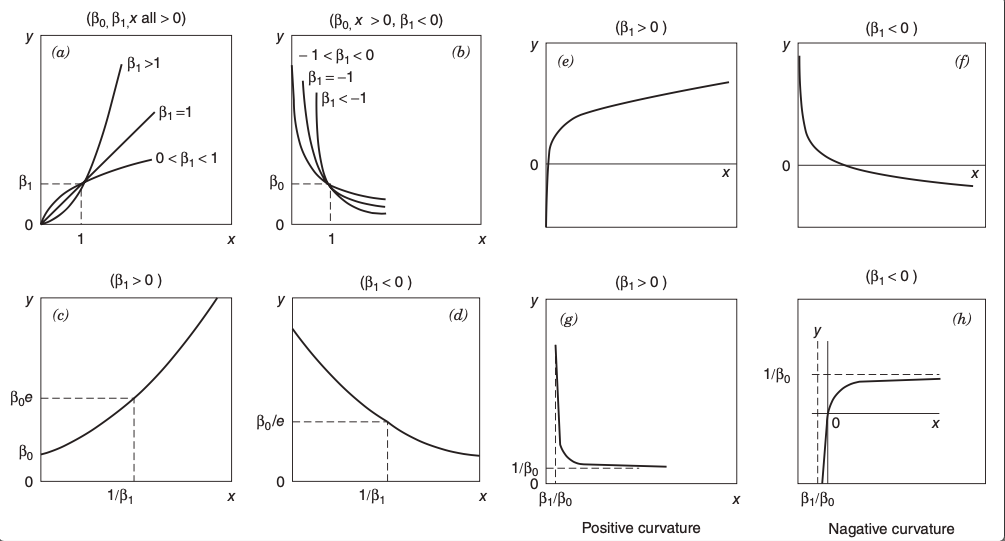
\includegraphics{images/Linealizables-01.png}
\caption{Funciones Linealizables}
\end{figure}

Otro ejemplo de modelos que podemos linealizar, son el caso de
transformaciones reciprocas, es decir algo de la forma

\[\dfrac{1}{y}=\beta_0+\beta_1 x+\varepsilon\] y
\[y=\dfrac{x}{\beta_0 x-\beta_1}+\epsilon\] \textbf{\emph{Comentario:}}
Cuando las transformaciones como las anteriores son empleadas el
estimador de mínimos cuadrados tiene propiedades de mínimos cuadrados
con respecto a los datos transformados, \textbf{\emph{no a los
originales}}.

\textbf{Ejemplo (Molino de Viento)}

\begin{Shaded}
\begin{Highlighting}[]
\NormalTok{tabla1 }\OtherTok{\textless{}{-}} \FunctionTok{data.frame}\NormalTok{(}\AttributeTok{stringsAsFactors=}\ConstantTok{FALSE}\NormalTok{,}
\AttributeTok{Velocidad\_Viento =} \FunctionTok{c}\NormalTok{(}\FloatTok{5.00}\NormalTok{, }\FloatTok{6.00}\NormalTok{, }\FloatTok{3.40}\NormalTok{, }\FloatTok{2.70}\NormalTok{,}
      \FloatTok{10.00}\NormalTok{, }\FloatTok{9.70}\NormalTok{, }\FloatTok{9.55}\NormalTok{, }\FloatTok{3.05}\NormalTok{, }\FloatTok{8.15}\NormalTok{, }\FloatTok{6.20}\NormalTok{, }\FloatTok{2.90}\NormalTok{, }\FloatTok{6.35}\NormalTok{, }\FloatTok{4.60}\NormalTok{, }\FloatTok{5.80}\NormalTok{, }\FloatTok{7.40}\NormalTok{, }\FloatTok{3.60}\NormalTok{,}
      \FloatTok{7.85}\NormalTok{, }\FloatTok{8.80}\NormalTok{, }\FloatTok{7.00}\NormalTok{, }\FloatTok{5.45}\NormalTok{, }\FloatTok{9.10}\NormalTok{, }\FloatTok{10.20}\NormalTok{, }\FloatTok{4.10}\NormalTok{, }\FloatTok{3.95}\NormalTok{, }\FloatTok{2.45}\NormalTok{),}
\AttributeTok{Salida\_DC =} \FunctionTok{c}\NormalTok{(}\FloatTok{1.582}\NormalTok{, }\FloatTok{1.822}\NormalTok{, }\FloatTok{1.057}\NormalTok{, }\FloatTok{0.500}\NormalTok{, }\FloatTok{2.236}\NormalTok{, }\FloatTok{2.386}\NormalTok{, }\FloatTok{2.294}\NormalTok{, }\FloatTok{0.558}\NormalTok{, }\FloatTok{2.166}\NormalTok{, }\FloatTok{1.866}\NormalTok{,}
     \FloatTok{0.653}\NormalTok{, }\FloatTok{1.930}\NormalTok{, }\FloatTok{1.562}\NormalTok{, }\FloatTok{1.737}\NormalTok{, }\FloatTok{2.088}\NormalTok{, }\FloatTok{1.137}\NormalTok{, }\FloatTok{2.179}\NormalTok{, }\FloatTok{2.112}\NormalTok{, }\FloatTok{1.800}\NormalTok{, }\FloatTok{1.501}\NormalTok{, }\FloatTok{2.303}\NormalTok{,}
     \FloatTok{2.310}\NormalTok{, }\FloatTok{1.194}\NormalTok{, }\FloatTok{1.144}\NormalTok{, }\FloatTok{0.123}\NormalTok{)}
\NormalTok{)}
\FunctionTok{names}\NormalTok{(tabla1)}\OtherTok{\textless{}{-}}\FunctionTok{c}\NormalTok{(}\StringTok{"Velocidad del Viento (Mph)"}\NormalTok{,}\StringTok{"Salida DC"}\NormalTok{)}
\NormalTok{tabla1}
\end{Highlighting}
\end{Shaded}

\begin{verbatim}
##    Velocidad del Viento (Mph) Salida DC
## 1                        5.00     1.582
## 2                        6.00     1.822
## 3                        3.40     1.057
## 4                        2.70     0.500
## 5                       10.00     2.236
## 6                        9.70     2.386
## 7                        9.55     2.294
## 8                        3.05     0.558
## 9                        8.15     2.166
## 10                       6.20     1.866
## 11                       2.90     0.653
## 12                       6.35     1.930
## 13                       4.60     1.562
## 14                       5.80     1.737
## 15                       7.40     2.088
## 16                       3.60     1.137
## 17                       7.85     2.179
## 18                       8.80     2.112
## 19                       7.00     1.800
## 20                       5.45     1.501
## 21                       9.10     2.303
## 22                      10.20     2.310
## 23                       4.10     1.194
## 24                       3.95     1.144
## 25                       2.45     0.123
\end{verbatim}

Un ingeniero, está investigando el uso de un molino de viento para
generar electricidad. Ha recopilado datos sobre la salida de DC de su
molino de viento y la velocidad del viento correspondiente. La
inspección del diagrama de dispersión indica que la relación entre la
salida de DC \((y)\) y la velocidad del viento \((x)\) puede ser no
lineal como veremos a continuación del gráfico de dispersión.

\begin{Shaded}
\begin{Highlighting}[]
\FunctionTok{plot}\NormalTok{(tabla1}\SpecialCharTok{$}\StringTok{\textasciigrave{}}\AttributeTok{Velocidad del Viento (Mph)}\StringTok{\textasciigrave{}}\NormalTok{,tabla1}\SpecialCharTok{$}\StringTok{\textasciigrave{}}\AttributeTok{Salida DC}\StringTok{\textasciigrave{}}\NormalTok{,}\AttributeTok{xlab=}\FunctionTok{TeX}\NormalTok{(r}\StringTok{\textquotesingle{}(Velocidad del Viento $x$ )\textquotesingle{}}\NormalTok{),}\AttributeTok{ylab=}\FunctionTok{TeX}\NormalTok{(r}\StringTok{\textquotesingle{}(Salida DC $y$)\textquotesingle{}}\NormalTok{),}\AttributeTok{pch=}\DecValTok{20}\NormalTok{,}\AttributeTok{cex=}\DecValTok{2}\NormalTok{)}
\end{Highlighting}
\end{Shaded}

\includegraphics{Seccion5_3_files/figure-latex/unnamed-chunk-3-1.pdf}

\begin{Shaded}
\begin{Highlighting}[]
\FunctionTok{mult.norm}\NormalTok{(tabla1)}\SpecialCharTok{$}\NormalTok{test}
\end{Highlighting}
\end{Shaded}

\begin{verbatim}
## NULL
\end{verbatim}

Como se puede observar del gráfico de dispersión, pareciera que la
relación entre la salida del voltaje en función de la velocidad del
viento es no lineal. Lo cual podemos contrastar con el trafico de
residuales.

Para ellos,a justando un modelo lineal obtenemos

\begin{Shaded}
\begin{Highlighting}[]
\NormalTok{modelo1}\OtherTok{\textless{}{-}}\FunctionTok{lm}\NormalTok{(tabla1}\SpecialCharTok{$}\StringTok{\textasciigrave{}}\AttributeTok{Salida DC}\StringTok{\textasciigrave{}}\SpecialCharTok{\textasciitilde{}}\NormalTok{tabla1}\SpecialCharTok{$}\StringTok{\textasciigrave{}}\AttributeTok{Velocidad del Viento (Mph)}\StringTok{\textasciigrave{}}\NormalTok{)}
\FunctionTok{summary}\NormalTok{(modelo1)}
\end{Highlighting}
\end{Shaded}

\begin{verbatim}
## 
## Call:
## lm(formula = tabla1$`Salida DC` ~ tabla1$`Velocidad del Viento (Mph)`)
## 
## Residuals:
##      Min       1Q   Median       3Q      Max 
## -0.59869 -0.14099  0.06059  0.17262  0.32184 
## 
## Coefficients:
##                                     Estimate Std. Error t value Pr(>|t|)    
## (Intercept)                          0.13088    0.12599   1.039     0.31    
## tabla1$`Velocidad del Viento (Mph)`  0.24115    0.01905  12.659 7.55e-12 ***
## ---
## Signif. codes:  0 '***' 0.001 '**' 0.01 '*' 0.05 '.' 0.1 ' ' 1
## 
## Residual standard error: 0.2361 on 23 degrees of freedom
## Multiple R-squared:  0.8745, Adjusted R-squared:  0.869 
## F-statistic: 160.3 on 1 and 23 DF,  p-value: 7.546e-12
\end{verbatim}

\begin{Shaded}
\begin{Highlighting}[]
\FunctionTok{shapiro.test}\NormalTok{(modelo1}\SpecialCharTok{$}\NormalTok{residuals)}
\end{Highlighting}
\end{Shaded}

\begin{verbatim}
## 
##  Shapiro-Wilk normality test
## 
## data:  modelo1$residuals
## W = 0.93587, p-value = 0.1188
\end{verbatim}

\begin{Shaded}
\begin{Highlighting}[]
\FunctionTok{plot}\NormalTok{(modelo1}\SpecialCharTok{$}\NormalTok{fitted.values,modelo1}\SpecialCharTok{$}\NormalTok{residuals,}\AttributeTok{pch=}\DecValTok{19}\NormalTok{,}\AttributeTok{xlab=}\StringTok{"Ajustado"}\NormalTok{,}\AttributeTok{ylab=}\StringTok{"Residuales"}\NormalTok{)}
\end{Highlighting}
\end{Shaded}

\includegraphics{Seccion5_3_files/figure-latex/unnamed-chunk-5-1.pdf}

\begin{Shaded}
\begin{Highlighting}[]
\FunctionTok{qqnorm}\NormalTok{(}\AttributeTok{y=}\NormalTok{modelo1}\SpecialCharTok{$}\NormalTok{residuals)}
\FunctionTok{qqline}\NormalTok{(modelo1}\SpecialCharTok{$}\NormalTok{residuals)}
\end{Highlighting}
\end{Shaded}

\includegraphics{Seccion5_3_files/figure-latex/unnamed-chunk-5-2.pdf}

Este comportamiento observado, hace pensar que en efecto el modelo
lineal no es el adecuado y quizás un modelo cuadrático del tipo
\[y=\beta_0+\beta_1 x+\beta_2 x^2+\varepsilon\] resulte mejor para
explicar la curvatura aparente. Sin embargo podemos observar del
diagrama de dispersión que a medida que la velocidad del viento aumenta,
la salida de voltaje se acerca un punto extremo de 2.5 , lo cual es
consistente con el funcionamiento de un molino de viento. Dado que el
modelo cuadrático eventualmente se doblará, esto indicaría que a
velocidades mas altas de este punto máximo observado la salida de
voltaje disminuiría lo cual, con lo cual nuevamente el modelo cuadrático
tampoco seria adecuado para los datos.

Como mencionamos a medida que la velocidad aumenta, la salida de voltaje
pareciera alcanzar un punto extremo, de manera que tiende como a
estabilizarse, lo que sugiere que una transformación de tipo reciproca
sea lo mas adecuada, pues en ellas incorporamos asíntotas, y en este
caso buscamos que haya una asíntota superior que se acerque a este valor
extremo. Transformando el modelo como
\[y=\beta_0+\beta_1 \left(\dfrac{1}{x}\right)+\varepsilon.\] Usando esta
transformación veamos su relación mediante el gráfico de dispersión

\begin{Shaded}
\begin{Highlighting}[]
\FunctionTok{plot}\NormalTok{(}\DecValTok{1}\SpecialCharTok{/}\NormalTok{tabla1}\SpecialCharTok{$}\StringTok{\textasciigrave{}}\AttributeTok{Velocidad del Viento (Mph)}\StringTok{\textasciigrave{}}\NormalTok{,tabla1}\SpecialCharTok{$}\StringTok{\textasciigrave{}}\AttributeTok{Salida DC}\StringTok{\textasciigrave{}}\NormalTok{,}\AttributeTok{xlab=}\FunctionTok{TeX}\NormalTok{(r}\StringTok{\textquotesingle{}(Velocidad del Viento $x$ )\textquotesingle{}}\NormalTok{),}\AttributeTok{ylab=}\FunctionTok{TeX}\NormalTok{(r}\StringTok{\textquotesingle{}(Salida DC $y$)\textquotesingle{}}\NormalTok{),}\AttributeTok{pch=}\DecValTok{20}\NormalTok{,}\AttributeTok{cex=}\DecValTok{2}\NormalTok{)}
\end{Highlighting}
\end{Shaded}

\includegraphics{Seccion5_3_files/figure-latex/unnamed-chunk-6-1.pdf}

\begin{Shaded}
\begin{Highlighting}[]
\NormalTok{ynuevos}\OtherTok{\textless{}{-}}\NormalTok{(tabla1}\SpecialCharTok{$}\StringTok{\textasciigrave{}}\AttributeTok{Salida DC}\StringTok{\textasciigrave{}}\NormalTok{)}\SpecialCharTok{\^{}}\DecValTok{2}
\CommentTok{\#plot(tabla1$\textasciigrave{}Velocidad del Viento (Mph)\textasciigrave{},ynuevos)}
\CommentTok{\#modelo22\textless{}{-}lm(ynuevos\textasciitilde{}tabla1$\textasciigrave{}Velocidad del Viento (Mph)\textasciigrave{})}
\CommentTok{\#plot(modelo22)}

\NormalTok{xnuevos}\OtherTok{\textless{}{-}}\FunctionTok{log}\NormalTok{(tabla1}\SpecialCharTok{$}\StringTok{\textasciigrave{}}\AttributeTok{Velocidad del Viento (Mph)}\StringTok{\textasciigrave{}}\NormalTok{)}
\NormalTok{modelo222}\OtherTok{\textless{}{-}}\FunctionTok{lm}\NormalTok{(tabla1}\SpecialCharTok{$}\StringTok{\textasciigrave{}}\AttributeTok{Salida DC}\StringTok{\textasciigrave{}}\SpecialCharTok{\textasciitilde{}}\NormalTok{xnuevos)}
\FunctionTok{plot}\NormalTok{(modelo222)}
\end{Highlighting}
\end{Shaded}

\includegraphics{Seccion5_3_files/figure-latex/unnamed-chunk-6-2.pdf}
\includegraphics{Seccion5_3_files/figure-latex/unnamed-chunk-6-3.pdf}
\includegraphics{Seccion5_3_files/figure-latex/unnamed-chunk-6-4.pdf}
\includegraphics{Seccion5_3_files/figure-latex/unnamed-chunk-6-5.pdf}
Ajustando el modelo, tenemos como resultado

\begin{Shaded}
\begin{Highlighting}[]
\NormalTok{tabla2 }\OtherTok{\textless{}{-}} \FunctionTok{data.frame}\NormalTok{(}\AttributeTok{stringsAsFactors=}\ConstantTok{FALSE}\NormalTok{,}
\AttributeTok{Velocidad\_Viento =} \DecValTok{1}\SpecialCharTok{/}\FunctionTok{c}\NormalTok{(}\FloatTok{5.00}\NormalTok{, }\FloatTok{6.00}\NormalTok{, }\FloatTok{3.40}\NormalTok{, }\FloatTok{2.70}\NormalTok{,}
      \FloatTok{10.00}\NormalTok{, }\FloatTok{9.70}\NormalTok{, }\FloatTok{9.55}\NormalTok{, }\FloatTok{3.05}\NormalTok{, }\FloatTok{8.15}\NormalTok{, }\FloatTok{6.20}\NormalTok{, }\FloatTok{2.90}\NormalTok{, }\FloatTok{6.35}\NormalTok{, }\FloatTok{4.60}\NormalTok{, }\FloatTok{5.80}\NormalTok{, }\FloatTok{7.40}\NormalTok{, }\FloatTok{3.60}\NormalTok{,}
      \FloatTok{7.85}\NormalTok{, }\FloatTok{8.80}\NormalTok{, }\FloatTok{7.00}\NormalTok{, }\FloatTok{5.45}\NormalTok{, }\FloatTok{9.10}\NormalTok{, }\FloatTok{10.20}\NormalTok{, }\FloatTok{4.10}\NormalTok{, }\FloatTok{3.95}\NormalTok{, }\FloatTok{2.45}\NormalTok{),}
\AttributeTok{Salida\_DC =} \FunctionTok{c}\NormalTok{(}\FloatTok{1.582}\NormalTok{, }\FloatTok{1.822}\NormalTok{, }\FloatTok{1.057}\NormalTok{, }\FloatTok{0.500}\NormalTok{, }\FloatTok{2.236}\NormalTok{, }\FloatTok{2.386}\NormalTok{, }\FloatTok{2.294}\NormalTok{, }\FloatTok{0.558}\NormalTok{, }\FloatTok{2.166}\NormalTok{, }\FloatTok{1.866}\NormalTok{,}
     \FloatTok{0.653}\NormalTok{, }\FloatTok{1.930}\NormalTok{, }\FloatTok{1.562}\NormalTok{, }\FloatTok{1.737}\NormalTok{, }\FloatTok{2.088}\NormalTok{, }\FloatTok{1.137}\NormalTok{, }\FloatTok{2.179}\NormalTok{, }\FloatTok{2.112}\NormalTok{, }\FloatTok{1.800}\NormalTok{, }\FloatTok{1.501}\NormalTok{, }\FloatTok{2.303}\NormalTok{,}
     \FloatTok{2.310}\NormalTok{, }\FloatTok{1.194}\NormalTok{, }\FloatTok{1.144}\NormalTok{, }\FloatTok{0.123}\NormalTok{)}
\NormalTok{)}
\FunctionTok{names}\NormalTok{(tabla2)}\OtherTok{\textless{}{-}}\FunctionTok{c}\NormalTok{(}\StringTok{"Velocidad del Viento (Mph)"}\NormalTok{,}\StringTok{"Salida DC"}\NormalTok{)}
\NormalTok{tabla2}
\end{Highlighting}
\end{Shaded}

\begin{verbatim}
##    Velocidad del Viento (Mph) Salida DC
## 1                  0.20000000     1.582
## 2                  0.16666667     1.822
## 3                  0.29411765     1.057
## 4                  0.37037037     0.500
## 5                  0.10000000     2.236
## 6                  0.10309278     2.386
## 7                  0.10471204     2.294
## 8                  0.32786885     0.558
## 9                  0.12269939     2.166
## 10                 0.16129032     1.866
## 11                 0.34482759     0.653
## 12                 0.15748031     1.930
## 13                 0.21739130     1.562
## 14                 0.17241379     1.737
## 15                 0.13513514     2.088
## 16                 0.27777778     1.137
## 17                 0.12738854     2.179
## 18                 0.11363636     2.112
## 19                 0.14285714     1.800
## 20                 0.18348624     1.501
## 21                 0.10989011     2.303
## 22                 0.09803922     2.310
## 23                 0.24390244     1.194
## 24                 0.25316456     1.144
## 25                 0.40816327     0.123
\end{verbatim}

\begin{Shaded}
\begin{Highlighting}[]
\NormalTok{modelo2}\OtherTok{\textless{}{-}}\FunctionTok{lm}\NormalTok{(tabla2}\SpecialCharTok{$}\StringTok{\textasciigrave{}}\AttributeTok{Salida DC}\StringTok{\textasciigrave{}}\SpecialCharTok{\textasciitilde{}}\NormalTok{tabla2}\SpecialCharTok{$}\StringTok{\textasciigrave{}}\AttributeTok{Velocidad del Viento (Mph)}\StringTok{\textasciigrave{}}\NormalTok{)}
\FunctionTok{summary}\NormalTok{(modelo2)}
\end{Highlighting}
\end{Shaded}

\begin{verbatim}
## 
## Call:
## lm(formula = tabla2$`Salida DC` ~ tabla2$`Velocidad del Viento (Mph)`)
## 
## Residuals:
##      Min       1Q   Median       3Q      Max 
## -0.20547 -0.04940  0.01100  0.08352  0.12204 
## 
## Coefficients:
##                                     Estimate Std. Error t value Pr(>|t|)    
## (Intercept)                           2.9789     0.0449   66.34   <2e-16 ***
## tabla2$`Velocidad del Viento (Mph)`  -6.9345     0.2064  -33.59   <2e-16 ***
## ---
## Signif. codes:  0 '***' 0.001 '**' 0.01 '*' 0.05 '.' 0.1 ' ' 1
## 
## Residual standard error: 0.09417 on 23 degrees of freedom
## Multiple R-squared:   0.98,  Adjusted R-squared:  0.9792 
## F-statistic:  1128 on 1 and 23 DF,  p-value: < 2.2e-16
\end{verbatim}

\begin{Shaded}
\begin{Highlighting}[]
\FunctionTok{plot}\NormalTok{(modelo2}\SpecialCharTok{$}\NormalTok{fitted.values,}\FunctionTok{rstudent}\NormalTok{(modelo2),}\AttributeTok{pch=}\DecValTok{19}\NormalTok{,}\AttributeTok{xlab=}\StringTok{"Ajustado"}\NormalTok{,}\AttributeTok{ylab=}\StringTok{"Residuales"}\NormalTok{)}
\FunctionTok{abline}\NormalTok{(}\AttributeTok{h=}\DecValTok{0}\NormalTok{,}\AttributeTok{lty=}\DecValTok{2}\NormalTok{,}\AttributeTok{col=}\StringTok{"red"}\NormalTok{)}
\end{Highlighting}
\end{Shaded}

\includegraphics{Seccion5_3_files/figure-latex/unnamed-chunk-9-1.pdf}

\begin{Shaded}
\begin{Highlighting}[]
\FunctionTok{plot}\NormalTok{(modelo2)}
\end{Highlighting}
\end{Shaded}

\includegraphics{Seccion5_3_files/figure-latex/unnamed-chunk-9-2.pdf}
\includegraphics{Seccion5_3_files/figure-latex/unnamed-chunk-9-3.pdf}
\includegraphics{Seccion5_3_files/figure-latex/unnamed-chunk-9-4.pdf}
\includegraphics{Seccion5_3_files/figure-latex/unnamed-chunk-9-5.pdf}

\begin{Shaded}
\begin{Highlighting}[]
\FunctionTok{ggqqplot}\NormalTok{(modelo2}\SpecialCharTok{$}\NormalTok{residuals)}
\end{Highlighting}
\end{Shaded}

\includegraphics{Seccion5_3_files/figure-latex/unnamed-chunk-9-6.pdf}

\begin{Shaded}
\begin{Highlighting}[]
\CommentTok{\#mult.norm(tabla1)$mult.test}
\end{Highlighting}
\end{Shaded}

\hypertarget{ejemplo-datos-mariajuana}{%
\subparagraph{\texorpdfstring{\textbf{Ejemplo Datos
MariaJuana}}{Ejemplo Datos MariaJuana}}\label{ejemplo-datos-mariajuana}}

Veamos ahora si podemos aplicar alguna transformación al conjunto de
datos de Mariajuana. Recordemos que en este conjunto de datos teníamos
en esencia tres subconjuntos a causa de los tres cantidades que se
tenían para la dosis. De esta manera es conveniente trabajar con estos
tres subconjuntos. Recordemos que las transformaciones que vimos
previamente por ahora están limitadas a la regresión lineal simple, con
lo cual consideraremos la altura como función de precipitación o como
función de la temperatura.

\begin{Shaded}
\begin{Highlighting}[]
\DocumentationTok{\#\# Carga del conjunto de datos}
\NormalTok{maria}\OtherTok{\textless{}{-}}\FunctionTok{read.table}\NormalTok{(}\StringTok{"/Users/danimathud/Documents/GitHub/R\_projects/ModelosEstadisticos1/Datas/Mariajuana.txt"}\NormalTok{)}
\NormalTok{maria}
\end{Highlighting}
\end{Shaded}

\begin{verbatim}
##    Altura.en.cm Temperatura.en.C Precipitación.pluvial.mm Dosis.en.kg
## 1      6.161183         42.17968                 648.0880         0.0
## 2      6.562611         41.14369                 648.9561         1.0
## 3      7.984795         39.81303                 649.3143         1.5
## 4      6.085641         38.82369                 650.1878         1.0
## 5      8.331910         37.31728                 648.4499         0.0
## 6      5.384640         50.77178                 651.1442         1.5
## 7      7.325221         35.13389                 648.2409         1.0
## 8      8.437257         37.55082                 647.9298         0.0
## 9      6.766811         41.96831                 651.1736         1.5
## 10     7.070951         39.07220                 647.5905         1.0
## 11     5.546558         42.68823                 651.2447         1.5
## 12     5.342291         42.06190                 650.5362         1.5
## 13     4.830554         43.03624                 652.2311         0.0
## 14     6.146142         45.05066                 649.7400         1.0
## 15     4.695256         41.81368                 651.8118         1.5
## 16     5.903617         40.28123                 651.1099         1.0
## 17     6.523599         37.00209                 647.6135         1.0
## 18     5.531760         36.42398                 650.6579         1.5
## 19     8.317800         33.61859                 650.9954         1.5
## 20     6.986574         37.28374                 647.9602         1.5
## 21     6.578493         39.74421                 648.4756         0.0
## 22     6.309085         46.24505                 651.0684         1.5
## 23     6.709897         39.62118                 650.0479         1.5
## 24     6.679480         39.05956                 650.1705         1.5
## 25     6.478600         36.14557                 648.7000         1.5
## 26     5.697406         40.88020                 650.4503         1.5
## 27     6.695523         40.23396                 647.4958         1.0
## 28     7.151076         41.63649                 650.8740         1.5
## 29     5.672478         38.82360                 649.9546         1.0
## 30     7.956164         39.76030                 648.9310         1.5
\end{verbatim}

\begin{Shaded}
\begin{Highlighting}[]
\DocumentationTok{\#\# Filtrado}
\NormalTok{maria\_dosis0}\OtherTok{\textless{}{-}}\NormalTok{maria }\SpecialCharTok{\%\textgreater{}\%} \FunctionTok{filter}\NormalTok{(Dosis.en.kg}\SpecialCharTok{==}\DecValTok{0}\NormalTok{)}
\NormalTok{maria\_dosis0}
\end{Highlighting}
\end{Shaded}

\begin{verbatim}
##    Altura.en.cm Temperatura.en.C Precipitación.pluvial.mm Dosis.en.kg
## 1      6.161183         42.17968                 648.0880           0
## 5      8.331910         37.31728                 648.4499           0
## 8      8.437257         37.55082                 647.9298           0
## 13     4.830554         43.03624                 652.2311           0
## 21     6.578493         39.74421                 648.4756           0
\end{verbatim}

\begin{Shaded}
\begin{Highlighting}[]
\NormalTok{maria\_dosis1}\OtherTok{\textless{}{-}}\NormalTok{maria }\SpecialCharTok{\%\textgreater{}\%} \FunctionTok{filter}\NormalTok{(Dosis.en.kg}\SpecialCharTok{==}\DecValTok{1}\NormalTok{)}
\NormalTok{maria\_dosis1}
\end{Highlighting}
\end{Shaded}

\begin{verbatim}
##    Altura.en.cm Temperatura.en.C Precipitación.pluvial.mm Dosis.en.kg
## 2      6.562611         41.14369                 648.9561           1
## 4      6.085641         38.82369                 650.1878           1
## 7      7.325221         35.13389                 648.2409           1
## 10     7.070951         39.07220                 647.5905           1
## 14     6.146142         45.05066                 649.7400           1
## 16     5.903617         40.28123                 651.1099           1
## 17     6.523599         37.00209                 647.6135           1
## 27     6.695523         40.23396                 647.4958           1
## 29     5.672478         38.82360                 649.9546           1
\end{verbatim}

\begin{Shaded}
\begin{Highlighting}[]
\NormalTok{maria\_dosis15}\OtherTok{\textless{}{-}}\NormalTok{maria }\SpecialCharTok{\%\textgreater{}\%} \FunctionTok{filter}\NormalTok{(Dosis.en.kg}\SpecialCharTok{==}\FloatTok{1.5}\NormalTok{)}
\NormalTok{maria\_dosis15}
\end{Highlighting}
\end{Shaded}

\begin{verbatim}
##    Altura.en.cm Temperatura.en.C Precipitación.pluvial.mm Dosis.en.kg
## 3      7.984795         39.81303                 649.3143         1.5
## 6      5.384640         50.77178                 651.1442         1.5
## 9      6.766811         41.96831                 651.1736         1.5
## 11     5.546558         42.68823                 651.2447         1.5
## 12     5.342291         42.06190                 650.5362         1.5
## 15     4.695256         41.81368                 651.8118         1.5
## 18     5.531760         36.42398                 650.6579         1.5
## 19     8.317800         33.61859                 650.9954         1.5
## 20     6.986574         37.28374                 647.9602         1.5
## 22     6.309085         46.24505                 651.0684         1.5
## 23     6.709897         39.62118                 650.0479         1.5
## 24     6.679480         39.05956                 650.1705         1.5
## 25     6.478600         36.14557                 648.7000         1.5
## 26     5.697406         40.88020                 650.4503         1.5
## 28     7.151076         41.63649                 650.8740         1.5
## 30     7.956164         39.76030                 648.9310         1.5
\end{verbatim}

\begin{Shaded}
\begin{Highlighting}[]
\FunctionTok{par}\NormalTok{(}\AttributeTok{mfrow=}\FunctionTok{c}\NormalTok{(}\DecValTok{1}\NormalTok{,}\DecValTok{3}\NormalTok{))}
\FunctionTok{plot}\NormalTok{(maria\_dosis0[,}\DecValTok{1}\SpecialCharTok{:}\DecValTok{3}\NormalTok{],}\AttributeTok{lower.panel=}\ConstantTok{NULL}\NormalTok{,}\AttributeTok{main=}\StringTok{"Dosis 0"}\NormalTok{)}
\end{Highlighting}
\end{Shaded}

\includegraphics{Seccion5_3_files/figure-latex/unnamed-chunk-12-1.pdf}

\begin{Shaded}
\begin{Highlighting}[]
\FunctionTok{par}\NormalTok{(}\AttributeTok{mfrow=}\FunctionTok{c}\NormalTok{(}\DecValTok{1}\NormalTok{,}\DecValTok{3}\NormalTok{))}
\FunctionTok{plot}\NormalTok{(maria\_dosis1[,}\DecValTok{1}\SpecialCharTok{:}\DecValTok{3}\NormalTok{],}\AttributeTok{lower.panel=}\ConstantTok{NULL}\NormalTok{,}\AttributeTok{main=}\StringTok{"Dosis 1"}\NormalTok{)}
\end{Highlighting}
\end{Shaded}

\includegraphics{Seccion5_3_files/figure-latex/unnamed-chunk-12-2.pdf}

\begin{Shaded}
\begin{Highlighting}[]
\FunctionTok{par}\NormalTok{(}\AttributeTok{mfrow=}\FunctionTok{c}\NormalTok{(}\DecValTok{1}\NormalTok{,}\DecValTok{3}\NormalTok{))}
\FunctionTok{plot}\NormalTok{(maria\_dosis15[,}\DecValTok{1}\SpecialCharTok{:}\DecValTok{3}\NormalTok{],}\AttributeTok{lower.panel=}\ConstantTok{NULL}\NormalTok{,}\AttributeTok{main=}\StringTok{"Dosis 1.5"}\NormalTok{)}
\end{Highlighting}
\end{Shaded}

\includegraphics{Seccion5_3_files/figure-latex/unnamed-chunk-12-3.pdf}

\begin{Shaded}
\begin{Highlighting}[]
\CommentTok{\#plot(maria[,1:3],lower.panel=NULL)}
\CommentTok{\#plot3d(maria[,1:3])}
\end{Highlighting}
\end{Shaded}

Para este ejemplo consideremos el subconjunto para dosis de 1.5, y
veamos para cual resulta mas conveniente una transformación, si para
altura en función de temperatura o altura en función de precipitación.

\textbf{Altura en función de la temperatura}

\begin{Shaded}
\begin{Highlighting}[]
\NormalTok{modelo3}\OtherTok{\textless{}{-}}\FunctionTok{lm}\NormalTok{(maria\_dosis15}\SpecialCharTok{$}\NormalTok{Altura.en.cm}\SpecialCharTok{\textasciitilde{}}\NormalTok{maria\_dosis15}\SpecialCharTok{$}\NormalTok{Temperatura.en.C)}
\FunctionTok{plot}\NormalTok{(modelo3,}\AttributeTok{pch=}\DecValTok{19}\NormalTok{)}
\end{Highlighting}
\end{Shaded}

\includegraphics{Seccion5_3_files/figure-latex/unnamed-chunk-13-1.pdf}
\includegraphics{Seccion5_3_files/figure-latex/unnamed-chunk-13-2.pdf}
\includegraphics{Seccion5_3_files/figure-latex/unnamed-chunk-13-3.pdf}
\includegraphics{Seccion5_3_files/figure-latex/unnamed-chunk-13-4.pdf}

\begin{Shaded}
\begin{Highlighting}[]
\FunctionTok{shapiro.test}\NormalTok{(modelo3}\SpecialCharTok{$}\NormalTok{residuals)}
\end{Highlighting}
\end{Shaded}

\begin{verbatim}
## 
##  Shapiro-Wilk normality test
## 
## data:  modelo3$residuals
## W = 0.96296, p-value = 0.7156
\end{verbatim}

\begin{Shaded}
\begin{Highlighting}[]
\FunctionTok{plot}\NormalTok{(maria\_dosis15}\SpecialCharTok{$}\NormalTok{Temperatura.en.C,maria\_dosis15}\SpecialCharTok{$}\NormalTok{Altura.en.cm,}\AttributeTok{xlab=}\StringTok{"Temperatura"}\NormalTok{,}\AttributeTok{ylab=}\StringTok{"Altura"}\NormalTok{,}\AttributeTok{pch=}\DecValTok{19}\NormalTok{)}
\FunctionTok{abline}\NormalTok{(modelo3,}\AttributeTok{col=}\StringTok{"red"}\NormalTok{)}
\end{Highlighting}
\end{Shaded}

\includegraphics{Seccion5_3_files/figure-latex/unnamed-chunk-13-5.pdf}

Como podemos considerando altura en función de temperatura, aunque del
gráfico de residuales y QQ pareciera que se cumplen todos los supuestos
de regresión lineal y normalidad en los errores, sin embargo podemos ver
también, que la recta no se ajusta lo suficientemente bien. Por lo cual
podríamos intentar transformar los datos esperando conseguir un mejor
resultado en el ajuste del modelo.

Notemos de los datos que la recta que ajustemos tiene parámetro
\(\beta_1<0\) y la temperatura que consideramos es positiva, con lo cual
podemos observar que nuestros datos, tienen mas parecido con los
gráficos b) y d) de la figura mostrada en un inició, así podríamos
intentar considerar como transformaciones

\[\log{y}=\log{\beta_0 x^{\beta_1}}=\log{\beta_0}+\beta_1\log{x}\] o
\[\log{y}=\log{\beta_0 e^{\beta_1 x}}=\log{\beta_0}+\beta_1 x.\] Veamos
cual de estas nos da buenos resultados

\begin{Shaded}
\begin{Highlighting}[]
\NormalTok{y1\_tran}\OtherTok{\textless{}{-}}\FunctionTok{log}\NormalTok{(maria\_dosis15}\SpecialCharTok{$}\NormalTok{Altura.en.cm)}
\NormalTok{x1\_tran}\OtherTok{\textless{}{-}}\FunctionTok{log}\NormalTok{(maria\_dosis15}\SpecialCharTok{$}\NormalTok{Temperatura.en.C)}
\FunctionTok{plot}\NormalTok{(x1\_tran,y1\_tran,}\AttributeTok{pch=}\DecValTok{19}\NormalTok{,}\AttributeTok{main=}\FunctionTok{TeX}\NormalTok{(r}\StringTok{\textquotesingle{}("Transformando con $y\textquotesingle{}}\OtherTok{=}\NormalTok{\textbackslash{}log\{(y)\}}\SpecialCharTok{$}\NormalTok{ y }\SpecialCharTok{$}\NormalTok{x}\StringTok{\textquotesingle{}=\textbackslash{}log\{(x)\}$)\textquotesingle{}}\NormalTok{),}\AttributeTok{xlab=}\StringTok{"log(Temperatura)"}\NormalTok{,}\AttributeTok{ylab=}\StringTok{"log(Altura)"}\NormalTok{)}
\NormalTok{modelo3\_tran1}\OtherTok{\textless{}{-}}\FunctionTok{lm}\NormalTok{(y1\_tran}\SpecialCharTok{\textasciitilde{}}\NormalTok{x1\_tran)}
\FunctionTok{abline}\NormalTok{(modelo3\_tran1,}\AttributeTok{col=}\StringTok{"blue"}\NormalTok{)}
\end{Highlighting}
\end{Shaded}

\includegraphics{Seccion5_3_files/figure-latex/unnamed-chunk-14-1.pdf}

\begin{Shaded}
\begin{Highlighting}[]
\FunctionTok{plot}\NormalTok{(modelo3\_tran1,}\AttributeTok{pch=}\DecValTok{19}\NormalTok{)}
\end{Highlighting}
\end{Shaded}

\includegraphics{Seccion5_3_files/figure-latex/unnamed-chunk-14-2.pdf}
\includegraphics{Seccion5_3_files/figure-latex/unnamed-chunk-14-3.pdf}
\includegraphics{Seccion5_3_files/figure-latex/unnamed-chunk-14-4.pdf}
\includegraphics{Seccion5_3_files/figure-latex/unnamed-chunk-14-5.pdf}

\begin{Shaded}
\begin{Highlighting}[]
\FunctionTok{shapiro.test}\NormalTok{(modelo3\_tran1}\SpecialCharTok{$}\NormalTok{residuals)}
\end{Highlighting}
\end{Shaded}

\begin{verbatim}
## 
##  Shapiro-Wilk normality test
## 
## data:  modelo3_tran1$residuals
## W = 0.96199, p-value = 0.6981
\end{verbatim}

\begin{Shaded}
\begin{Highlighting}[]
\FunctionTok{plot}\NormalTok{(maria\_dosis15}\SpecialCharTok{$}\NormalTok{Temperatura.en.C,y1\_tran,}\AttributeTok{pch=}\DecValTok{19}\NormalTok{,}\AttributeTok{main=}\FunctionTok{TeX}\NormalTok{(r}\StringTok{\textquotesingle{}("Transformando con $y\textquotesingle{}}\OtherTok{=}\NormalTok{\textbackslash{}log\{(y)\}}\SpecialCharTok{$}\NormalTok{)}\StringTok{\textquotesingle{}),ylab="log(Altura)",xlab="Temperatura")}
\StringTok{modelo3\_tran2\textless{}{-}lm(y1\_tran\textasciitilde{}maria\_dosis15$Temperatura.en.C)}
\StringTok{abline(modelo3\_tran2,col="red")}
\end{Highlighting}
\end{Shaded}

\includegraphics{Seccion5_3_files/figure-latex/unnamed-chunk-15-1.pdf}

\begin{Shaded}
\begin{Highlighting}[]
\FunctionTok{plot}\NormalTok{(modelo3\_tran2,}\AttributeTok{pch=}\DecValTok{19}\NormalTok{)}
\end{Highlighting}
\end{Shaded}

\includegraphics{Seccion5_3_files/figure-latex/unnamed-chunk-15-2.pdf}
\includegraphics{Seccion5_3_files/figure-latex/unnamed-chunk-15-3.pdf}
\includegraphics{Seccion5_3_files/figure-latex/unnamed-chunk-15-4.pdf}
\includegraphics{Seccion5_3_files/figure-latex/unnamed-chunk-15-5.pdf}

\begin{Shaded}
\begin{Highlighting}[]
\FunctionTok{shapiro.test}\NormalTok{(modelo3\_tran2}\SpecialCharTok{$}\NormalTok{residuals)}
\end{Highlighting}
\end{Shaded}

\begin{verbatim}
## 
##  Shapiro-Wilk normality test
## 
## data:  modelo3_tran2$residuals
## W = 0.95863, p-value = 0.637
\end{verbatim}

\end{document}
